% =========================================================================== %

\begin{frame}[t,plain]
\titlepage
\end{frame}

% =========================================================================== %

\begin{frame}{Recap}
%
\begin{columns}[T]
\column{.5\linewidth}
\begin{itemize}
\item Advanced forms of argument lists
	\begin{itemize}
	\item Optional arguments
	\item Variadic functions
	\item Keyword arguments
	\end{itemize}
\item Returning functions
	\begin{itemize}
	\item Return a reference
	\item Function generators
	\end{itemize}
\end{itemize}
%
\column{.5\linewidth}
\begin{itemize}
\item Lambdas
	\begin{itemize}
	\item Shorthand form for functions
	\item Often used as arguments (\thus \texttt{sort})
	\end{itemize}
\item Recursion
	\begin{itemize}
	\item Functions calling themselves
	\item Solution to self-similar problems
	\item \enquote{Boxes} with variables of their own
	\end{itemize}
\end{itemize}

\end{columns}
%
\begin{center}
	\emph{Any Questions?}
\end{center}
%
\end{frame}

% =========================================================================== %
\begin{frame}[fragile]{Seen in the Exercises}
%
\begin{codebox}[Lambda as a key]
\begin{minted}[fontsize=\scriptsize, linenos]{python}
data = [(9, 1), (8, 2), (7, 3), (6, 4), (5, 5)]
print( sorted(data, key=lambda x: x[0]**2 + x[1]**2) )
\end{minted}
\end{codebox}
%
\begin{itemize}
\item Lambda: Projection \inPy{tuple} \thus Length
\item Called for each \inPy{tuple} in the \inPy{list data}
\item Sort by length, ascendingly 
\end{itemize}
%
\end{frame}

% =========================================================================== %

\begin{frame}[fragile]
%
\begin{codebox}[Binary Search \emph{with} Rekursion]
\begin{minted}[fontsize=\scriptsize, linenos]{python}
def binarySearch (data, searchTerm) :
  size = len(data)
  
  if (size == 1) :
    if data[0] == searchTerm : return True
    else                     : return False
  else :
    midPoint = size // 2
    if   data[midPoint] == searchTerm : return True
    elif data[midPoint]  < searchTerm : return binarySearch(data[midPoint:], searchTerm)
    else                              : return binarySearch(data[:midPoint], searchTerm)

data = [1, 5, 6, 7, 8, 42, 96, 666, 1337, 2112]
searchTerm = 42

print("### binarySearch")
print(binarySearch(data, searchTerm) , end="\n\n")      # test for middle element
print(binarySearch(data, 1)          , end="\n\n")      # test for first element
print(binarySearch(data, 2112)       , end="\n\n")      # test for last element
print(binarySearch(data, 2)          , end="\n\n")      # test for not in list
\end{minted}
\end{codebox}
%
\end{frame}

% =========================================================================== %

\begin{frame}[fragile]
%
\begin{codebox}[Binary Search \emph{without} Rekursion]
\begin{minted}[fontsize=\scriptsize, linenos]{python}
def midSearch(data, searchTerm):
    first = 0
    last  = len(data)
    index = -1
    
    while(first <= last) and (index == -1):
        mid = (first+last) // 2
        if data[mid] == searchTerm:
            index = mid
        else:
            if searchTerm < data[mid]: last  = mid - 1
            else                     : first = mid + 1

    if index == -1: print("Element not in list")
    else          : return index

data = [1, 5, 6, 7, 8, 42, 96, 1337, 2112]
print(midSearch(data, 1337))
\end{minted}
\end{codebox}
%
\begin{flushright}
\scriptsize \emph{Thanks to Michael Briehl for this code}
\end{flushright}
%
\end{frame}

% =========================================================================== %

\begin{frame}[fragile]{Chapter 7}
%
\begin{itemize}
\item Classes as Data Containers
\item Methods
\item Magic methods (\enquote{dunders})
\end{itemize}
%
\end{frame}

% =========================================================================== %

\begin{frame}{Classes}
%
\begin{itemize}
\item Idea: Computer \enquote{knows} only numbers (integers)
\item Only interpreting these numbers yields texts, pictures, programs, ...
\item Example: 98, 108, 117, 101
	\begin{itemize}
	\item ASCII-Codes for characters \texttt{b, l, u, e}?
	\item or street numbers of the adresses of my first four girlfriends?
	\item \emph{Context} necessary for interpretation!
	\end{itemize}
\item Classes: Data object with attached context
	\begin{itemize}
	\item Collection of values
	\item Methods for interpreting these values
	\end{itemize}
\item Usually: \emph{similar} Objects \Thus name \emph{classes}
\end{itemize}
%
\end{frame}

% =========================================================================== %

\begin{frame}[fragile]{Classes in Python -- Data Types}
%
\begin{columns}[T]
\column{.5\linewidth}
\begin{itemize}
\item Data types in Python are examples of classes
	\begin{itemize}
	\item Example: \inPy{list}s
	\item \enquote{Data content}: liste elements
	\item Assigned methods: sort, reverse, append, ...
	\item \texttt{append} makes no sense with an \inPy{int}!
	\end{itemize}
\item Designing classes means: creating your own data type
\item Internally: composition of known data types
\end{itemize}
%
\column{.5\linewidth}
\begin{codebox}[Syntax: Creating Classes]
\begin{minted}[fontsize=\scriptsize]{python}
class ClassName :
    # Definitions
\end{minted}
\end{codebox}

\begin{codebox}[Syntax: Instantiating a Class]
\begin{minted}[fontsize=\scriptsize]{python}
newVar = ClassName()
\end{minted}
\end{codebox}
\begin{itemize}
\item Infinite possiblities for \texttt{Definitions}
\item Most important details in this lecture
\end{itemize}
\end{columns}
%
\end{frame}

% =========================================================================== %

\begin{frame}{Who had it worse?}
%
\begin{center}
\scriptsize
\textbf{Stefan's romantic past}
\rowcolors{1}{tabhighlight}{tabcontrast}
\begin{tabular}{c|ccp{.3\linewidth}p{.3\linewidth}}
	\textbf{Symbol} & \textbf{Name} & \textbf{Height} & \textbf{Upsides}                                 & \textbf{Downsides} \tabcrlf
	\texttt{exgf1}  & Steffie       & 1.65 m          & intelligent, beautiful, has a dog                & too attached to her mother, 
																																																				doesn't like meeting people \\
	\texttt{exgf2}  & Epsi          & 1.63 m          & very intelligent, beautiful, good taste in music & doesn't like coffee, doesn't like coding \\
	\texttt{exgf3}  & Katja         & 1.81 m          & intelligent, very beautiful, musician            & moody, cheated on me
\end{tabular}
\end{center}

\begin{center}
\scriptsize
\textbf{Charlotte's broken hearts}
\rowcolors{1}{tabhighlight}{tabcontrast}
\begin{tabular}{c|ccp{.3\linewidth}p{.3\linewidth}}
	\textbf{Symbol} & \textbf{Name} & \textbf{Height} & \textbf{Upsides}                                 & \textbf{Downsides} \tabcrlf
	\texttt{exbf1}  & Sebastian     & 1.78 m          & intelligent, handsome, likes to listen           & obsessed with catching bugs, always late \\
	\texttt{exbf2}  & Reginald      & 1.84 m          & very intelligent, handsome, plays in a band      & flirty with everyone, complains a lot \\
	\texttt{exbf3}  & Sönke         & 1.81 m          & intelligent, quite handsome, cheerful nature     & superficial, racist
\end{tabular}
\end{center}
%
\end{frame}

% =========================================================================== %

\begin{frame}[fragile]{Classes as Pure Containers}
%
\begin{codebox}[Syntax: Class with \emph{Attributes}]
\begin{minted}[fontsize=\scriptsize]{python}
class ClassName :
    attribute1 = value1
    attribute2 = value2
    ...
\end{minted}
\end{codebox}
%
\begin{codebox}[Syntax: Accessing Attributes]
\begin{minted}[fontsize=\scriptsize]{python}
instance = ClassName()

instance.attribute1 = newValue
ClassName.attribute1 = newValue

instance.newAttribute = newValue
ClassName.newAttribute = newValue
\end{minted}
\end{codebox}
%
\end{frame}

% =========================================================================== %

\begin{frame}[fragile]
%
\begin{codebox}[Example: Changing Attributes]
\begin{minted}[fontsize=\scriptsize, linenos]{python}
class Cla :
    bar = "dead parrot"
    lst = [1]

foo = cla()
\end{minted}
\end{codebox}
%
\begin{tcbraster}[raster columns=2,
                  raster equal height,
                  nobeforeafter,
                  raster column skip=0.5cm]
\begin{codebox}[(... continued ...)]
\begin{minted}[fontsize=\scriptsize, linenos, firstnumber=last]{python}
print("via foo:", foo.bar)
print("via Cla:", Cla.bar, end="\n\n")
cla.bar = "lumberjack"
print("via foo:", foo.bar)
print("via Cla:", Cla.bar, end="\n\n")
foo.bar = "hovercraft"
print("via foo:", foo.bar)
print("via Cla:", Cla.bar, end="\n\n")
foo.new = "eel"
print("via foo:", foo.new, end="\n\n")
# print("via Cla:", Cla.new)
\end{minted}
\end{codebox}
%
\begin{cmdbox}[Output: Changing Attributes]
\begin{minted}[fontsize=\scriptsize]{text}
via foo: dead parrot
via Cla: dead parrot

via foo: lumberjack
via Cla: lumberjack

via foo: hovercraft
via Cla: lumberjack

via foo: eel
\end{minted}
\end{cmdbox}
\end{tcbraster}
%
\end{frame}

% =========================================================================== %

\begin{frame}[fragile]
%
\begin{tcbraster}[raster columns=2,
                  raster equal height,
                  nobeforeafter,
                  raster column skip=0.5cm]
\begin{codebox}[(... continued ...)]
\begin{minted}[fontsize=\scriptsize, linenos, firstnumber=20]{python}
# ...

foo.lst.append(2)
print("via foo:", foo.lst)
print("via Cla:", Cla.lst, end="\n\n")
\end{minted}
\end{codebox}
%
\begin{cmdbox}[(... continued ...)]
\begin{minted}[fontsize=\scriptsize]{text}
...


via foo: [1, 2]
via Cla: [1, 2]
\end{minted}
\end{cmdbox}
\end{tcbraster}
%
\vspace{15pt}
%
\begin{center}
	\Thus\,???
\end{center}
%
\end{frame}

% =========================================================================== %\\

\begin{frame}[fragile]
%
\begin{tcolorbox}[title=Memory Model]
Up to line 8 (only read access):
\begin{center}
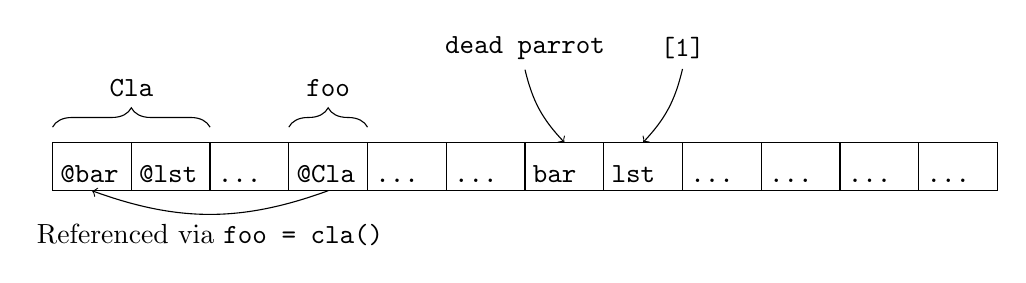
\begin{tikzpicture}
  [ 
    cell/.style={text width=8mm,
      text height=4mm, draw=black, inner sep=1mm},
    ld/.style={draw=blue,shorten >=2pt,->}
  ]
  \node  (a0) at ( 0,0) [cell] {\ttfamily @bar};
  \node  (a1) at ( 1,0) [cell] {\ttfamily @lst};
  \node  (a2) at ( 2,0) [cell] {\ttfamily ...};
  \node  (a3) at ( 3,0) [cell] {\ttfamily @Cla};
  \node  (a4) at ( 4,0) [cell] {\ttfamily ...};
  \node  (a5) at ( 5,0) [cell] {\ttfamily ...};
  \node  (a6) at ( 6,0) [cell] {\ttfamily bar};
  \node  (a7) at ( 7,0) [cell] {\ttfamily lst};
  \node  (a8) at ( 8,0) [cell] {\ttfamily ...};
  \node  (a9) at ( 9,0) [cell] {\ttfamily ...};
  \node (a10) at (10,0) [cell] {\ttfamily ...};
  \node (a11) at (11,0) [cell] {\ttfamily ...};
  
  \draw [decorate, decoration={brace,amplitude=7pt}, xshift=-0pt, yshift=0pt]
  		(-0.5, 0.5) -- ( 1.5, 0.5) node (x) [midway, yshift=+0.5cm] 
		(braceFuncDerivative) {\texttt{Cla}};
	
  \draw [decorate, decoration={brace,amplitude=7pt}, xshift=-0pt, yshift=0pt]
  		( 2.5, 0.5) -- ( 3.5, 0.5) node (y) [midway, yshift=+0.5cm] 
		(braceFuncDerivative) {\texttt{foo}};
	
	\draw [->, bend left=20]
		(a3.south) to node 
		[below] {Referenced via \texttt{foo = cla()}} 
		(a0.south);
		
	\node (t6) at (5.5,+1.5) {\texttt{dead parrot}};
	\node (t7) at (7.5,+1.5) {\texttt{[1]}};
	
	\draw [->, bend right=15] (t6.south) to node [below] {} (a6.north);
	\draw [->, bend left =15] (t7.south) to node [below] {} (a7.north);
\end{tikzpicture}
\end{center}
\texttt{foo} only holds a reference to \texttt{Cla}. This symbol, in turn, references \texttt{bar} and \texttt{lst}.
\end{tcolorbox}
%
\end{frame}

% =========================================================================== %\\

\begin{frame}[fragile]
%
\begin{tcolorbox}[title=Memory Model]
Line 10: \inPy{Cla.bar = "lumberjack"}
\begin{center}
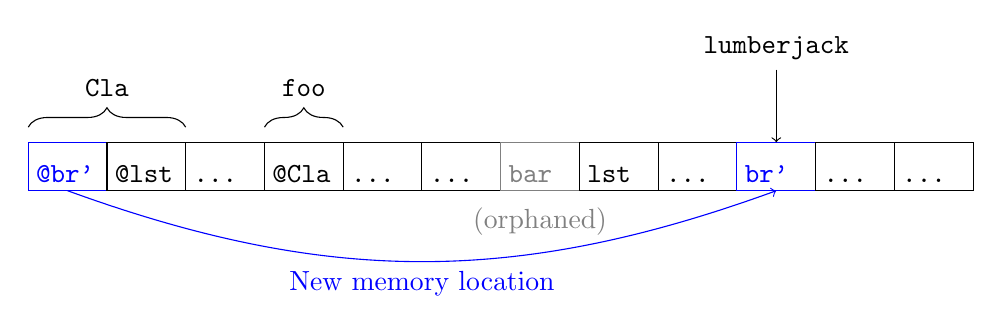
\begin{tikzpicture}
  [ 
    cell/.style={text width=8mm,
      text height=4mm, draw=black, inner sep=1mm},
    ld/.style={draw=blue,shorten >=2pt,->}
  ]
  \node  (a0) at ( 0,0) [cell, blue] {\ttfamily @br'};
  \node  (a1) at ( 1,0) [cell] {\ttfamily @lst};
  \node  (a2) at ( 2,0) [cell] {\ttfamily ...};
  \node  (a3) at ( 3,0) [cell] {\ttfamily @Cla};
  \node  (a4) at ( 4,0) [cell] {\ttfamily ...};
  \node  (a5) at ( 5,0) [cell] {\ttfamily ...};
  \node  (a6) at ( 6,0) [cell, gray] {\ttfamily bar};
  \node  (a7) at ( 7,0) [cell] {\ttfamily lst};
  \node  (a8) at ( 8,0) [cell] {\ttfamily ...};
  \node  (a9) at ( 9,0) [cell, blue] {\ttfamily br'};
  \node (a10) at (10,0) [cell] {\ttfamily ...};
  \node (a11) at (11,0) [cell] {\ttfamily ...};
  
  \draw [decorate, decoration={brace,amplitude=7pt}, xshift=-0pt, yshift=0pt]
  		(-0.5, 0.5) -- ( 1.5, 0.5) node (x) [midway, yshift=+0.5cm] 
		(braceFuncDerivative) {\texttt{Cla}};
	
  \draw [decorate, decoration={brace,amplitude=7pt}, xshift=-0pt, yshift=0pt]
  		( 2.5, 0.5) -- ( 3.5, 0.5) node (y) [midway, yshift=+0.5cm] 
		(braceFuncDerivative) {\texttt{foo}};
	
	\draw [->, bend right=20, blue]
		(a0.south) to node 
		[below] {New memory location} 
		(a9.south);
	
	\node (t6) at (6,-0.7) {\color{gray}(orphaned)};
	
	\node (t9) at (9,+1.5) {\texttt{lumberjack}};
	\draw [->] (t9.south) to node [below] {} (a9.north);
\end{tikzpicture}
\end{center}
Changes to \texttt{Cla} also affect \texttt{foo}, since this really is nothing but a reference to \texttt{Cla}.\\
Since \texttt{bar} is \emph{immutable} (property of strings), changes to \texttt{bar} only affect the new memory location; the old location becomes orphaned.
\end{tcolorbox}
%
\end{frame}

% =========================================================================== %\\

\begin{frame}[fragile]
%
\begin{tcolorbox}[title=Memory Model]
Line 14: \inPy{foo.bar = "hovercraft"}\\
Line 18: \inPy{foo.new = "eel"}
\begin{center}
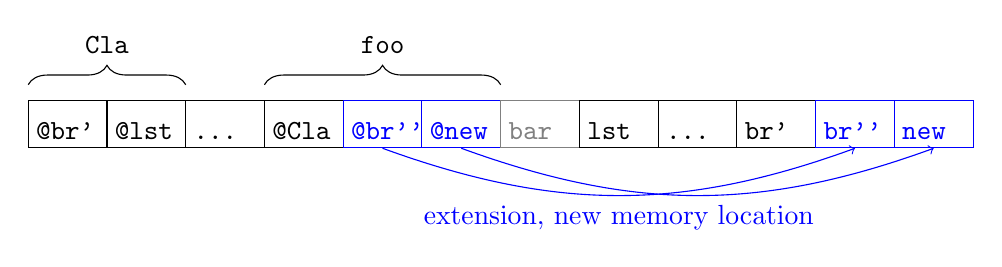
\begin{tikzpicture}
  [ 
    cell/.style={text width=8mm,
      text height=4mm, draw=black, inner sep=1mm},
    ld/.style={draw=blue,shorten >=2pt,->}
  ]
  \node  (a0) at ( 0,0) [cell] {\ttfamily @br'};
  \node  (a1) at ( 1,0) [cell] {\ttfamily @lst};
  \node  (a2) at ( 2,0) [cell] {\ttfamily ...};
  \node  (a3) at ( 3,0) [cell] {\ttfamily @Cla};
  \node  (a4) at ( 4,0) [cell, blue] {\ttfamily @br''};
  \node  (a5) at ( 5,0) [cell, blue] {\ttfamily @new};
  \node  (a6) at ( 6,0) [cell, gray] {\ttfamily bar};
  \node  (a7) at ( 7,0) [cell] {\ttfamily lst};
  \node  (a8) at ( 8,0) [cell] {\ttfamily ...};
  \node  (a9) at ( 9,0) [cell] {\ttfamily br'};
  \node (a10) at (10,0) [cell, blue] {\ttfamily br''};
  \node (a11) at (11,0) [cell, blue] {\ttfamily new};
  
  \draw [decorate, decoration={brace,amplitude=7pt}, xshift=-0pt, yshift=0pt]
  		(-0.5, 0.5) -- ( 1.5, 0.5) node (x) [midway, yshift=+0.5cm] 
		(braceFuncDerivative) {\texttt{Cla}};
	
  \draw [decorate, decoration={brace,amplitude=7pt}, xshift=-0pt, yshift=0pt]
  		( 2.5, 0.5) -- ( 5.5, 0.5) node (y) [midway, yshift=+0.5cm] 
		(braceFuncDerivative) {\texttt{foo}};
	
	\draw [->, bend right=20, blue]
		(a4.south) to node 
		[below] {extension, new memory location} 
		(a10.south);
	\draw [->, bend right=20, blue]
		(a5.south) to node 
		[below] {}
		(a11.south);
\end{tikzpicture}
\end{center}
The memory describing \texttt{foo} is extended to hold not only a reference to \texttt{Cla}, but also to new strings.  New memory is allocated for those strings.\\
Up to these amendments, the basic structure of \texttt{Cla} still holds: accessing \texttt{foo.lst} goes via \texttt{Cla.lst}.\\
Since \texttt{lst} is \emph{mutable} (property of \inPy{list}s), no new memory location is created in line 22 (\inPy{foo.lst.append(2)}).
\end{tcolorbox}
%
\end{frame}

% =========================================================================== %\\

\begin{frame}
%
\begin{hintbox}[Class Attributes and Instance Attributes]
We distinguish between attributes that are shared between all instances of a class and such that are specific for a particular instance.

Example Expartners: We want to judge all former partners by a common ruleset. This common ruleset could be a \emph{class attribute}.
On the other hand, the specific details of the former partners (traits, name, ...) are \emph{instance attributes}: All my ex-girlfriends had a name, but the name \emph{Epsi} is specific to one of them.

Class attributes are written \emph{within the class}. Instance attributes are defined at the instances themselves.
\end{hintbox}
%
\end{frame}

% =========================================================================== %

\begin{frame}[fragile]
%
\begin{codebox}[Example: Class Attributes and Instance Attributes]
\begin{minted}[linenos, fontsize=\scriptsize]{python}
class Expartner :
    traits = {
        "good taste in music"         :   2, "beautiful"                   :   3,
        "handsome"                    :   3, "intelligent"                 :   5,
        "very beautiful"              :   5, "very handsome"               :   5,
        "very intelligent"            :  10, "doesn't like coding"         : - 4,
        "doesn't like meeting people" : - 4, "complains a lot"             : - 8,
        "cheated on me"               : -20, "racist"                      : -30
    }

exgf2 = Expartner()
exgf2.name      = "Epsi"
exgf2.height    = 1.65
exgf2.upsides   = {"very intelligent", "beautiful", "good taste in music"}
exgf2.downsides = {"doesn't like coffee", "doesn't like coding"}

exbf2 = Expartner()
exbf2.name      = "Reginald"
exbf2.height    = 1.84
exbf2.upsides   = {"very intelligent", "handsome", "plays in a band"}
exbf2.downsides = {"flirty with everyone", "complains a lot"}
\end{minted}
\end{codebox}
%
\end{frame}

% =========================================================================== %

\begin{frame}[fragile]
%
\begin{columns}[T]
\column{.5\linewidth}
\begin{Large}
	{Classes with Methods}
	\vspace{6pt}
\end{Large}
\begin{itemize}
\item Method: Function that accesses data \enquote{in} an instance
\item Definition \emph{within the class}
\item Obligatory first argument: \inPy{self}
	\begin{itemize}
	\item Reference to the instance on which the method is called
	\item[\Thus] Access instance (and class attributes) via \inPy{self}
	\item Passed automatically when calling the method
	\item Name \inPy{self} is only a convention
	\end{itemize}
\item Each class has their own list of names
\end{itemize}
%
\column{.5\linewidth}
\begin{codebox}[Syntax: Defining a Method]
\begin{minted}[fontsize=\scriptsize]{python}
class ClassName :
    ...
    def method(self, ...) :
       Code
    ...
\end{minted}
\end{codebox}
%
\begin{codebox}[Syntax: Calling A Method]
\begin{minted}[fontsize=\scriptsize]{python}
Instance = ClassName()
Instance.method(...)
\end{minted}
\end{codebox}
%
\begin{itemize}
\item[\Thus] There may be two (or more) distinct classes, each of them having their own method called \texttt{doStuff}
\end{itemize}
\end{columns}
%
\end{frame}

% =========================================================================== %

\begin{frame}[fragile]
%
\begin{codebox}[Example: Class with Methods]
\begin{minted}[linenos, fontsize=\scriptsize]{python}
class Expartner :
    traits = { ... }   # as before
   
    def areThey(self, trait) :
        return (trait in self.upsides) or (trait in self.downsides)
    
    def rating(self) :
        reVal = 0
        for trait in self.upsides :
            if trait in self.traits : reVal += self.traits[trait]
            else                    : reVal += +1
        for trait in self.downsides :
            if trait in self.traits : reVal += self.traits[trait]
            else                    : reVal += -1
        return reVal

# exgf2, exbf2 as before

print( exgf2.areThey("very intelligent") )   # Output: True
print( exbf2.rating() )                      # Output: 5
\end{minted}
\end{codebox}
%
\end{frame}


% =========================================================================== %

\begin{frame}{Magic Methods (\enquote{Dunders})}
%
\begin{itemize}
\item Calls to functions: sometimes a lot to type, bad legibilty
	\begin{itemize}
	\item Compare: \inPy{x + y} with \inPy{x.add(y)}
	\end{itemize}
\item[\Thus] For most common operations: own mechanism
\item \enquote{Hidden} (automatic) function calls
	\begin{itemize}
	\item Initialization: \inPy{__init__}
	\item Computations: \inPy{__add__}, \inPy{__sub__}, \inPy{__mul__}, \inPy{__matmul__}, \inPy{__truediv__}, \inPy{__floordiv__}
	\item Comparisons: \inPy{__eq__}, \inPy{__ne__}, \inPy{__gt__}, \inPy{__ge__}, \inPy{__lt__}, \inPy{__le__}
	\item String representation: \inPy{__str__} und \inPy{__repr__}
	\item Use as a function: \inPy{__call__}
	\end{itemize}
\item \emph{Double Underscore} \Thus \enquote{Dunders}
\end{itemize}
%
\end{frame}

% =========================================================================== %

\begin{frame}[fragile]
%
\begin{columns}[T]
\column{.5\linewidth}
\begin{Large}
	{\inPy{__init__} -- Constructor (Initializer)}
\end{Large}
\vspace{6pt}
%
\begin{itemize}
\item Called as soon as an instance of a class is created
\item After \inPy{self}: free form (any number of arguments)
\item Usually: Put default values into the instance
\end{itemize}
%
\column{.5\linewidth}
\begin{codebox}[Syntax: \texttt{\_\_init\_\_}]
\begin{minted}[fontsize=\scriptsize]{python}
class ClassName :
    # class attributes
    
    def __init__ (self, ...) :
        ...
\end{minted}
\end{codebox}
%
\begin{codebox}[Syntax: Call to \texttt{\_\_init\_\_}]
\begin{minted}[fontsize=\scriptsize]{python}
instance = ClassName(...)
\end{minted}
\end{codebox}
\end{columns}
%
\end{frame}

% =========================================================================== %

\begin{frame}[fragile]
%
\begin{codebox}[Example: \texttt{\_\_init\_\_}]
\begin{minted}[linenos, fontsize=\scriptsize]{python}
class Expartner :
    # class attributes ...
    
    def __init__(self, name = None, height = None, upsides = {}, downsides = {}) :
        if height < 0 :
            raise Exception("Your Ex cannot be less than 0.0m tall")
        
        self.name      = name
        self.height    = height
        self.upsides   = upsides
        self.downsides = downsides
    
perfect = Expartner("Arista" , 1.70, 
              {"very intelligent", "very beautiful", "good taste in music"}
          )
\end{minted}
\end{codebox}
%
\end{frame}

% =========================================================================== %

\begin{frame}[fragile]{\inPy{__str__} and \inPy{__repr__} -- Text Representation}
%
\begin{columns}[T]
\column{.5\linewidth}
%
\begin{itemize}
\item Both methods: return text that represents the instance
\item \inPy{__str__}
	\begin{itemize}
	\item \enquote{End user form}, most commonly needed form
	\item Automatically called by \inPy{str(instance)}
	\item \inPy{print} automatically calls \inPy{str} for each non-string argument
	\end{itemize}
\item \inPy{__repr__}
	\begin{itemize}
	\item \emph{Debug form}, may be shorter or hold whatever you may need for development
	\item Automatisch called by \inPy{repr(instance)}
	\end{itemize}
\item Both methods take \textbf{no arguments}!
\end{itemize}
%
\column{.5\linewidth}
\begin{codebox}[Syntax: \texttt{\_\_str\_\_} and \texttt{\_\_repr\_\_}]
\begin{minted}[fontsize=\scriptsize]{python}
class ClassName :
    def __repr__ (self) :
        return someString
    
    def __str__ (self) :
        return someString
\end{minted}
\end{codebox}
%
\begin{codebox}[Syntax: Call \texttt{\_\_str\_\_} and \texttt{\_\_repr\_\_}]
\begin{minted}[fontsize=\scriptsize]{python}
instance = ClassName()

print(instance)         # beide
print(str(instance))    # gleich
pritn(repr(instance))
\end{minted}
\end{codebox}
\end{columns}
%
\end{frame}

% =========================================================================== %

\begin{frame}[fragile]{\inPy{__call__} -- Calling Instances as Functions}
%
\begin{columns}[T]
\column{.5\linewidth}
%
\begin{itemize}
\item Idea: Use a class instance as if it were a function
\item Could be useful for a game depending on lots of parameters:
	\begin{minted}{python}
	game = Game()
	game.playerCount = 2
	game.timeLimit   = 30
	...
	game()
	\end{minted}
\item Arbitrary count and kind of arguments
\end{itemize}
%
\column{.5\linewidth}
\begin{codebox}[Syntax: \texttt{\_\_call\_\_}]
\begin{minted}[fontsize=\scriptsize]{python}
class ClassName :
    def __call__ (self, ...) :
        ...
\end{minted}
\end{codebox}
%
\begin{codebox}[Syntax: Aufruf \texttt{\_\_call\_\_}]
\begin{minted}[fontsize=\scriptsize]{python}
Instance = ClassName()

Instance(...)
\end{minted}
\end{codebox}
\end{columns}
%
\end{frame}

% =========================================================================== %

\begin{frame}[fragile]
%
\begin{codebox}[Example: Calling an Instance]
\begin{minted}[linenos, fontsize=\scriptsize]{python}
class Expartner :
    # as before
    
    def __call__(self) :
        print("You shouldn't call your Ex'es. Leave the past behind.")

ex = Expartner("Sandra", 1.70)
ex()
\end{minted}
\end{codebox}
%
\end{frame}